\documentclass[12pt,a4paper,oneside]{article}

\usepackage[top=2.0cm, bottom=2.0cm, left=3cm, right=1.5cm, footskip=0.5cm]{geometry}

\usepackage{cmap}                               % Улучшенный поиск русских слов в полученном pdf-файле
\usepackage[T1,T2A]{fontenc}                    % Поддержка русских букв
\usepackage[utf8]{inputenc}[2014/04/30]         % Кодировка utf8
\usepackage[english, russian]{babel}[2014/03/24]% Языки: русский, английский

\usepackage{setspace}
\usepackage{graphicx}

\usepackage{array}
\usepackage{multirow}

\usepackage{xcolor}
\usepackage{listings}
\usepackage{ucs}

\usepackage{csquotes}
\usepackage{url}
\usepackage{filecontents}
\begin{filecontents}{mybib.bib}
\end{filecontents}

\usepackage{cite}

\definecolor{mGreen}{rgb}{0,0.6,0}
\definecolor{mGray}{rgb}{0.5,0.5,0.5}
\definecolor{mPurple}{rgb}{0.58,0,0.82}
\definecolor{backgroundColour}{rgb}{0.95,0.95,0.92}

\lstdefinestyle{CStyle}{
    backgroundcolor=\color{backgroundColour},   
    commentstyle=\color{mGreen},
    keywordstyle=\color{magenta},
    numberstyle=\tiny\color{mGray},
    stringstyle=\color{mPurple},
    basicstyle=\footnotesize,
    breakatwhitespace=false,         
    breaklines=true,                 
    captionpos=b,                    
    keepspaces=true,                 
    numbers=left,                    
    numbersep=5pt,                  
    showspaces=false,                
    showstringspaces=false,
    showtabs=false,                  
    tabsize=2,
    language=C
}
\lstset{inputencoding=utf8, extendedchars=\true}

\usepackage{amssymb}

\setstretch{1.25}
\begin{document}

\tableofcontents
\newpage

\section{Вступление}

\indent

% TODO: add reference: presentation EETimes
Встраиваемые системы получают всё большее распространение в современном мире. Примеры их использования можно найти почти в любой области деятельности, начиная от промышленных систем, сложной техники с множеством подобных устройств, автомобилей и летательных аппаратов и заканчивая обычными персональными устройствами наподобие мобильных телефонов или бытовой техники. В последнее время также набирает популярность интернет вещей (``Internet of Things'', IOT) -- область, связанная с использованием большого количества постоянно обменивающихся между собой информацией вычислительных устройств в самых различных направлениях деятельности\cite{EET}.

% TODO: add reference: presentation EETimes
Развитие области применения встраиваемых систем приводит к их постепенному усложнению, так как от таких устройств требуется всё больше функциональности. Необходимость расширения функционала приводит к потребности в увеличении производительности процессоров в таких системах, что влечёт за собой изменения в архитектуре и микроархитектуре, например, к добавлению кэшей и расширению набора инструкций. Таким образом процессоры в таких устройствах становятся всё более похожими на процессоры общего назначения, поэтому открываются новые возможности для оптимизации программного обеспечения, загружаемого во встраиваемые системы\cite{EET}.

% TODO: add reference: presentation EETimes
Расширение функционала устройств также приводит к изменениям в программном обеспечении встроенных систем. Оно становится всё более сложным и ресурсоёмким. Растёт количество строк в проектах, появляется всё больше уровней абстракции. Ручная оптимизация постепенно теряет приоритет, уступая его непосредственно написанию и проектированию сложного кода. При этом усложнение архитектуры открывает возможности для новых оптимизаций, поэтому с учётом того, что во встраиваемых системах особенно ценны ресурсы процессора, появляется необходимость в автоматическом проведении оптимизаций над кодом, например, с помощью компилятора\cite{EET}\cite{Complex}.

% TODO: add reference: misses
Современные приложения, как для процессоров общего назначения, так и для встраиваемых систем, могут очень активно использовать память, при этом частота работы процессоров выше, чем частота работы оперативной памяти, что может повлечь за собой задежки при исполнении инструкций (проблема, известная как ``Memory wall''). Эффективным средством борьбы с ними являются кэши, но даже хорошо спроектированная многоуровневая иерархия кэшей не позволяет полностью избавиться от задержек. Промахи в кэш будут происходить как при первичных доступах к данным, так и просто при нерегулярном доступе в память (например, при обходе дерева, узлы которого выделены в куче)\cite{Bour2010}\cite{Ferdman:2012}.

% TODO: add reference: about software prefetching
В качестве одного из решений данной проблемы можно привести поддержку компилятора, анализирующего доступы в память, и вставляющего специальные инструкции предподкачки данных в кэш. Однако при таком подходе встаёт вопрос о том, как определить, где действительно нужна трансформация, а где нет, так как сгенерированный код в последнем случае либо не делает никакой полезной работы, либо загрязняет кэш, что может приводить к ухудшению производительности. В случае же успешной предподкачки исполнение программ может значительно ускоряться, показывая хорошие результаты на различных классах приложений\cite{MemAcc}.

% add ref
В современных компиляторах уже существуют решения, использующие разные алгоритмы для предподкачки данных. Однако в компиляторах с открытым исходным кодом ещё реализованы далеко не все оптимизации, какие хотелось бы видеть пользователю. Например, в компиляторах GCC\cite{GCCPref} и LLVM есть только трансформация для обычных проходов по массивам.

\newpage

\section{Цель работы}

\indent

Главной целью данного проекта является разработка машинно-независимой оптимизирующей трансформации предподкачки данных для циклов в открытой инфраструктуре компилятора LLVM. В рамках данной работы можно выделить пять основных частей, которые, в свою очередь, также охватывают несколько различных областей в соответствующих темах. Первые две составляющие являются исследовательской работой, остальное -- сама разработка и тестирование полученной фазы.

\paragraph{Исследование алгоритмов}

В данной части необходимо исследовать нескольких подходов для различных способов работы с памятью, таких как косвенные доступы и доступы к рекурсивным структурам данных, представляющим наибольший интерес ввиду отсутвия какой-либо регулярности при доступе в память.

\paragraph{Исследование компиляторов}

Вторая часть работы должна включать в себя исследование уже существующих решений в различных компиляторах на предмет их возможностей касательно данной оптимизации, а также возможности настройки поведения фаз.

\paragraph{Разработка фаз}

Третья часть -- непосредственно разработка комплексной трансформации, состоящей из четырёх отдельных подзадач:
\begin{itemize}
\item разработка фазы архитектурно-зависимой преаллокации (только для архитектуры ARC);
\item улучшение уже существующей фазы для предподкачки данных при регулярных доступах (\textbf{``stride accesses''}) -- добавление предподкачки перед циклом и возможности предподкачки во внешних циклах;
\item разработка фазы предподкачки данных для косвенных доступов (\textbf{``indirect accesses''});
\item разработка фазы предподкачки данных для доступов в рекурсивных структурах данных (\textbf{``recursive data structures''}, \textbf{``RDS''}).
\end{itemize}

\paragraph{Добавление опций}

Параллельно с разработкой фаз появляется необходимость дать пользователю возможность контролировать поведение трансформации. Для этого на основе проведённых во второй части исследований в компилятор добавляются:

\begin{itemize}
\item опции, контролирующие поведение фазы в целом -- в течение всей компиляции модуля;
\item прагмы, контролирующие поведение фазы на уровне циклов;
\item атрибуты функций, контролирующие поведение фазы только для конкретной процедуры.
\end{itemize}

\paragraph{Тестирование фаз}

Заключительная часть работы состоит из отладки и тестирования внесённых в компилятор изменений для повышения стабильности трансформации и проверки её применимости к различным видам кода.

\section{Существующие решения}

\indent

Прежде чем приступить непосредственно к разработке, необходимо провести анализ существующих алгоритмов в литературе и публикациях и решений в современных компиляторах. Стоит отметить, что сама реализация каких-либо алгоритмов в проприетарных компиляторах с закрытым кодом обычно представляет собой чёрный ящик ввиду отсутствия доступа к исходному коду. Поэтому рассматривается только пользовательский интерфейс, предоставленный для управления параметрами оптимизаций.

\subsection{Алгоритмы}

\indent

% add reference to classification
Перед рассмотрением самих алгоритмов предподкачки данных стоит выделить виды доступов в память, потому что методы для предподкачки данных для разных типов обращений будут существенно отличаться друг от друга. Все приложения по типу доступов в память можно классифицировать следующим образом\cite{LeeMemClass}. Во-первых, доступы в память могут быть \emph{регулярными} (например, проход по массиву) и \emph{нерегулярными} (хэш-таблицы, деревья, выделенные в куче). Во-вторых, нерегулярные доступы далее можно разделить ещё на две категории: доступ по указателям в \emph{рекурсивных структурах данных} и доступ через \emph{косвенную адресацию} (например, один массив индексируется значениями другого). Первое разбиение позволяет разделить приложения, активно использующие память, на \emph{регулярные} и \emph{нерегулярные}. Краткая сводка этой классификации дана в таблице. Аппаратные методы обозначены \textbf{HW}, программные -- \textbf{SW}.

\begin{table}[h]
  \begin{center}
    \begin{tabular}{|| m{4cm} | l | l | m{5.5cm} ||}
      \hline
      Тип доступа & Пример кода & \multicolumn{2}{|l|}{Способы борьбы с задержками} \\
      \hline\hline
      \multirow{2}{4cm}{Регулярный доступ} & \texttt{a[i] = /* ... */} & HW & Потоковый буфер \\ \cline{3-4}
                  &  \texttt{a[i * 2] = /* ... */} & SW & Предподкачка массивов в циклах \\
      \hline
      Косвенный доступ & \texttt{x = a[b[i]];} & SW & Предподкачка для косвенных доступов с подгрузкой промежуточных индексов \\
      \hline
      \multirow{4}{4cm}{Рекурсивные структуры данных} & \multirow{4}{*}{\texttt{list = list->next;}} & HW & Предподкачка на основе зависимостей \\ \cline{3-4}
                  & & \multirow{3}{*}{SW} & Жадная предподкачка \\
                  & & & Предподкачка линеаризацией данных \\
                  & & & Предподкачка по запомненным указателям \\
      \hline
    \end{tabular}
    \caption{Классификация доступов в память}
    \label{tab:classify}
  \end{center}
\end{table}

На тему предподкачки данных существует много различных публикаций, относящихся как к программной реализации предподкачки в компиляторах, так и к решениям на микроархитектурном уровне. В данной работе фокус направлен на программные методы оптимизации, однако также изучены и решения на уровне микроархитектуры, влияющие на необходимость применения трансформаций компилятором.

\subsubsection{Регулярные доступы}

% TODO: add reference to prefetch instr proposal, Callahan 1991, Mowry 1992
\paragraph{Программная предподкачка данных}

Добавление предподкачки для регулярных доступов является довольно простой и интуитивно понятной трансформацией. Эта оптимизация рассматривается вместе с внедрением самой инструкции для предподкачки\cite{CallahanPref}, так как регулярные доступы имеют хорошую пространственную локальность, поэтому предподкачка в данном случае даст выигрыш, если нет дополнительных устройств в самом процессоре. Алгоритм для такой оптимизации можно посмотреть, например, в работах\cite{MowryStride}\cite{CallahanPref}.

\paragraph{Аппаратная поддержка предподкачки}

% add ref to stream buffers
Одно из решений на уровне микроархитектуры процессора -- это добавление \emph{потокового буфера} (``Stream buffer'')\cite{Jouppi:1990}, специального устройства, организованного в виде очереди (``FIFO buffer'') и позволяющего предподкачивать данные при промахах в кэш. При таком подходе используется свойство пространственной локальности, так как данные начинают спекулятивно подкачиваться по адресам, идущим после адреса, по которому был промах. Сам потоковый буфер стоит между кэшом первого уровня и кэшом второго уровня (или памятью), при этом процессор также соединён с буфером, чтобы у него была возможность сравнивать тэги записей. Дополнительное улучшение потокового буфера заключается в том, что делается несколько таких буферов, чтобы у них была возможность подкачивать данные из разных областей памяти одновременно (например, такое необходимо при обработке нескольких массивов в циклах). Такой буфер называется \emph{многоканальным потоковым буфером} (``Multi-way stream buffer'').

Алгоритм работы такого устройства можно описать следующим образом. Когда происходит промах в кэш первого уровня, потоковый буфер начинает последовательно подкачивать данные из кэша верхнего уровня, начиная с адреса, по которому был промах. Для каждого запроса в буфере создаётся соответствующая запись, хранящая тэг для запрашиваемого адреса. Когда данные приходят от верхнего уровня, они кладутся в буфер в соответсвии сохранённым тэгом. При этом в кэш первого уровня ничего не записывается, чтобы не загрязнять его данными, которые, возможно, не будут использованы. Затем, если процессор запрашивает данные из памяти, сравниваются тэги не только в кэше, но и в потоковом буфере. Если в потоковом буфере нашлась запись, то она перемещается в кэш, а остальные записи сдвигаются, освобождая место. При новом промахе весь буфер начинает работу заново.

\subsubsection{Рекурсивные структуры данных}

\indent

Рекурсивные структуры данных широко используются в приложениях общего назначения\cite{LukPhd}. Простейшим видом такой структуры является односвязный список, каждый узел которого выделен в динамической памяти (куче). При этом все элементы, кроме последнего, ссылаются последовательно друг на друга. При обходе подобного списка в циклах получается, что при каждом доступе к узлу может происходить промах в кэше, потому что нет какой-то чёткой структуры расположения элементов списка в памяти. Другими примерами рекурсивных структур данных являются деревья и графы. Обход таких объектов осуществляется по более сложным правилам.

\begin{figure}
  \centering
  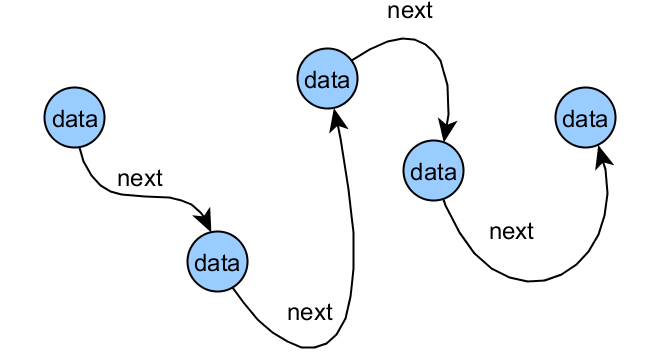
\includegraphics[width=0.9\textwidth]{rds.PNG}
  \caption{Пример рекурсивной структуры данных}
\end{figure}


В данной работе исследовалось несколько способов предподкачки данных для рекурсивных структур. Один из них включает изменения в микроархитектуре и добавлении новых блоков в процессор, три других -- программные методы разной степени сложности в реализации.

\paragraph{Предподкачка на основе зависимостей}

\emph{Предподкачка на основе зависимостей} (``Dependency-based prefetching'')\cite{Roth:1998} является динамическим методом и реализуется на уровне микроархитектуры процессора. Во время исполнения программы анализируются чтения из памяти и на основе полученной информации строятся предположения о том, как связаны между собой адреса и инструкции. Затем из полученных данных определяется, что необходимо подкачивать в кэш для будущего использования. Таким образом этот блок распознаёт обходы рекурсивных структур данных и подкачивает следующие элементы.

Метод использует четыре новые структуры. Первые две отвечают за построение связей между инструкциями и адресами, по которым они что-либо загружают. Оставшиеся две уже непосредственно реализуют механизм предподкачки.

Построение связей между инструкциями происходит при помощи \emph{таблицы корреляции} (``Correlation Table'') и \emph{таблицы возможных производителей} (``Potential Producer Window''). Таблица корреляций содержит в себе пары счётчиков команд производителей и потребителей адреса, а также шаблон для генерации такого адреса. Чтобы эта таблица постепенно наполнялась, используется таблица возможных производителей. Каждый раз, когда завершается исполнение какой-либо инструкции чтения из памяти (то есть на стадии ``commit''), то сначала адрес, по которому происходило чтение, проверяется на наличие в ТВП, а затем туда же записывается счётчик команд и загруженный этой инструкцией значение. Таким образом, ТВП содержит в себе записи из адреса и счётчик команд. Если адрес нашёлся в ТВП, то добавляется запись в ТК.

Далее используется \emph{очередь запросов на предподкачку} (``Prefetch Request Queue''), запись в которую заносится, если после завершения инструкции чтения из памяти её адрес нашёлся в КТ. Запись в ОЗП содержит счётчик команд потребителя из соответствующей записи КТ и адрес для предподкачки, который получается применением шаблона к загруженным данным. После того, как запись сформировалась, идёт ожидание, пока освободятся порты памяти. Затем отправляется запрос на предподкачку и добавляется запись в \emph{буфер предподкачки} (``Prefetch Buffer''), который содержит в себе счётчик команд потребителя, адрес и загруженное из памяти значение. Затем при исполнении потребителя обращение идёт одновременно к кэшу и к буферу предподкачки. Если в буфере находится значение, то оно используется инструкцией, а запись используется далее для генерации следующего адреса.

% ref to mowry, chi
\paragraph{Методы поиска рекурсивных структур данных}

Переходя к программным методам предподкачки данных в случае рекурсивных структур, следует отметить, что при статическом анализе программы появляется гораздо больше информации, чем при динамическом. В первую очередь для анализа доступов к указателям в рекурсивных структурах данных при компиляции исходного кода становятся известны типы указателей. Таким образом можно гораздо проще и точнее определять рекурсивные доступы.

В литературе\cite{LukPhd} существует алгоритм, позволяющий определить, является ли тип рекурсивной структурой данных. В его основе лежит поиск указателей на другие структуры внутри анализируемого типа. Делается проход по полям структуры и среди них ищутся указатели или массивы. Как только находится подобный тип, начинается вычисление того, на какой тип ссылается данный указатель или объекты какого типа содержит в себе массив. Происходит постепенное разыменовывание типа, в конце концов, приводящее к получению уже не указателя, а какого-то конкретного типа. Если этот тип -- структура, то считается, что исходный анализируемый тип является рекурсивной структурой данных. В противном случае анализ продолжается на оставшихся полях. Если поля заканчиваются, то структура не рекурсивная.

\paragraph{Естественные и искусственные указатели}

Стоит обратить внимание на то, что оптимизирующие трансформации могут быть очень агрессивными и, например, довольно сильно менять исходный код, типы и расположение данных. В программных методах предподкачки для рекурсивных структур проведено достаточно много исследований, что влечёт за собой некоторое разнообразие алгоритмов для решения задачи. Среди них есть и агрессивные оптимизации, дополняющие структуры данных новыми полями.

Методы предподкачки для рекурсивных структур используют информацию, содержащуюся в самих этих объектах. То есть, например, при проходе по списку инструкция предподкачки выполняется для адреса, полученного каким-либо образом из доступного внутри структуры указателя (в данном случае из указателя на следующий элемент списка). Способ, которым такой адрес получается из исходного указателя, называется \emph{функцией получения адреса}\cite{LukPhd}\cite{LukRDS}. Формально, если $A_i$ -- текущий адрес, $d$ -- дистанция для предподкачки, достаточная, чтобы скрыть задержки, и $A_{i+d}$ -- адрес элемента, который необходимо вычислить, а $\mathcal{F}$ -- функция получения адреса, то:
\begin{displaymath}
  A_{i+d} = \mathcal{F}(A_i,d).
\end{displaymath}

Указатель $A_i$ называется \emph{указателем перехода} (``Jump-pointer''). Такие указатели внутри рекурсивных структур данных подразделяют на два типа. Первый тип называется \emph{естественным} (``natural''). Под естественностью этих указателей подразумевается то, что они появились в программе без участия компилятора -- только потому что сам программист определил структуры данных таким образом. Второй тип -- это \emph{искусственные} (``artificial'') указатели. Это указатели, которые появились в структуре в результате проведения каких-либо оптимизаций компилятором. Такие указатели затем используются в модифицированных процедурах, которые каким-либо образом могут использовать эту информацию или же перезаписывать значения этих новых полей. Такая классификация удобна для последующего анализа алгоритмов программной предподкачки.

\paragraph{Жадная предподкачка}

Относительно простым методом среди всех способов предподкачки доступов к рекурсивным структурам является \emph{жадная предподкачка} (``Greedy prefetching''). Её жадность заключается в том, что при анализе какого-либо участка программы, например, цикла или рекурсивных вызовов процедур, ищутся все использованные естественные указатели в структуре. Затем, в зависимости от функции получения адреса, добавляются инструкции предподкачки по полученным адресам.

Стоит заметить, что несмотря на простоту, такой подход является довольно эффективным и хорошо справляющимся с уменьшением задержек доступов в память. Например, при обходе дерева, у каждого узла которого $k$ потомков, задежка полностью пропадает при доступе к $\frac{k-1}{k}$ узлам. То есть для бинарного дерева примерно 50\% узлов будет вовремя подкачано в кэш.

\paragraph{Проблема погони за указателем}

В предыдущем алгоритме не было уточнения о том, какой именно должна быть функция $\mathcal{F}$. Обозначим количество разыменований при вычислении следующего адреса с помощью $\mathcal{F}$ как $||\mathcal{F}||$. Очевидно, что при жадной предподкачке $||\mathcal{F}||$ не может быть нулевым. Случай, когда $||\mathcal{F}|| = 1$ является довольно ожидаемым -- при таком подходе всегда предподкачиваются только ближайшие узлы (например, следующий элемент списка), так как есть только одно разыменование. Дополнительно можно заметить, что для данной схемы $||\mathcal{F}|| = d$.

Теперь остался случай, когда $||\mathcal{F}|| > 1$. То есть количество разыменований становится больше, благодаря чему появляется возможность получить, например, $i+2$-ой элемент списка при наличии только указателя на $i$-ый элемент. Однако такой подход оказывается нерабочим, так как для разыменовывания последующих указателей приходится ждать, пока подкачается предыдущий элемент. Эта проблема известна под названием \emph{проблемы погони за указателем} (``Pointer-chasing problem''). Из-за этой проблемы получается, что в более чем одном разыменовании при жадной предподкачке нет никакого смысла. Наглядное доказательство этого утверждения можно посмотреть, например, в презентации\cite{MowryChasing}.

\paragraph{Предподкачка по запомненным указателям}

Следующим методом предподкачки при рекусивных доступах является \emph{предподкачка по запомненным указателям} (``History-pointer prefetching''). Этот метод пытается решить проблему погони за указателем с помощью введения дополнительного искусственного указателя в структуру данных. Этот указатель используется при обходах структуры, чтобы получать адрес необходимого для предподкачки элемента за одно разыменование. То есть при таком подходе получается, что $d > 1$ и $||\mathcal{F}|| = 0$.

Сам алгоритм отличается своей сложностью, так как требуется довольно большая работа по модификации кода программы. Во-первых, необходимо добавить в структуры особые искуственные указатели, называющиеся \emph{запоминающие указатели} (``History-pointer''). Во-вторых, потребуется добавить код для инициализации этих указателей, причём для каждого вида рекурсивной структуры данных будет собственный метод, что уже создаёт определённые сложности при анализе структур и процедур, которые их обрабатывают. В-третьих, появляется возможность того, что все указатели придётся перевязывать на другие элементы в случае модификации всего объекта.

Таким образом, предподкачка по запомненным адресам является очень эффективным методом в плане сокрытия задержек, если программа редко модифицирует рекурсивные структуры. В качестве отрицательных сторон выступают очень высокая сложность реализации, большие расходы во время исполнения при часто меняющихся объектах, на которые была применена оптимизация, и дополнительный расход памяти для содержания запоминающих указателей.

\paragraph{Предподкачка линеаризацией данных}

Последний рассмотренный в работе метод, посвящённый проблеме предподкачки для рекурсивных структур, использует в качестве функции получения адреса линейную аппроксимацию. То есть,

\begin{displaymath}
  A_{i+d} = A_i + d \times sizeof(A_0).
\end{displaymath}

Благодаря такому подходу в \emph{предподкачке линеаризацией данных} (``Data-linearization prefetching'') достигается очень грубая оценка адреса следующего элемента. При этом получается, что $||\mathcal{F}|| = 0$, то есть адрес $i+d$-го элемента вычисляется без каких-либо разыменований вообще. Данная схема опирается на факт, что элементы рекурсивной структуры данных могут быть расположены в динамической памяти примерно последовательно. Однако такое маловероятно при обычном распределении динамической памяти, поэтому появляется идея, связанная с перестановкой и уплотнением выделенных элементов для того, чтобы получить выигрыш от пространственной локальности. Однако сама процедура уплотнения может быть очень дорогой во время исполнения. Также необходимо заботиться о том, чтобы в программе не оставалось указателей на старые адреса памяти, уже не являющиеся действительными после перестановки.

% Работа товарищей из Кембриджа
\subsubsection{Косвенные доступы}

\indent

Следующей важной частью исследования является обзор алгоритмов, посвящённых проблемам предподкачки при косвенных доступах к данным. Эта тема, по сравнению с предыдущей, не получила широкого распространения, однако, учитывая то, что это один из трёх основных способов работы с памятью, она также должна быть рассмотрена в рамках данной работы.

В качестве примера для разбора взят алгоритм для косвенных доступов в циклах\cite{AinsworthIA}, в котором предподкачка идёт по нескольким массивам сразу -- и индексирующему, и индексируемому. В простом примере \texttt{ x += a[b[i]] } массив \texttt{a} -- индексируемый, массив \texttt{b} -- индексирующий. Исследование показывает, что при подобном доступе требуются две предподкачки.

\lstinputlisting[caption=Пример предподкачки для косвенного доступа в память, style=CStyle]{indirect_example.c}

Сам же алгоритм состоит из трёх основных этапов. Сначала идёт поиск в глубину всех подходящих цепочек по графу зависимости по данным. Поиск прекращается, если найдена индуктивная переменная (успешный результат, цепочка запоминается) или если найден инвариант цикла (в таком случае ничего запоминать не надо). Затем убираются лишние цепочки, усложняющие анализ. Например, цепочка со сложной зависимостью от фи-узлов или с вызовом функции будет отброшена. Затем наступает фаза генерации кода предподкачки. Начинается проход по найденным цепочкам. Для каждой инструкции загрузки из памяти копируется часть цепочки, оканчивающаяся именно этой инструкцией. Эта часть используется, чтобы сгенерировать адрес отстоящего на некоторой дистанции элемента из соответствующего массива. Затем вместо самой инструкции чтения добавляется инструкция предподкачки данных.

Более подробно алгоритм будет рассмотрен в секции, посвящённой реализации преобразований.

% kim 2002
\subsubsection{Другие методы}

\indent

Последний метод, который будет упомянут в работе, нельзя отнести ни к одной из предыдущих категорий, потому что он может покрывать различные типы доступа в память. В этом методе используется \emph{предысполнение при помощи компилятора} (``Compiler-based pre-execution'')\cite{Kim}, благодаря которому происходит предподкачка данных в память.

Основным элементом в данной трансформации является \emph{срез программы} (``Program slice''), представляющий собой некоторый участок программы. Так как эта оптимизация статическая, то весь анализ происходит на уровне исходного кода, в отличие от динамических схем, просматривающих уже инструкции процессора. Интересующие участки программы анализируются на возможность \emph{срезки} (``Slicing''), то есть клонирования кода и удалению из него инструкций, модифицирующих глобальное состояние программы (например, изменения глобальных переменных или запись по указателю в динамическую память). Также в новую функцию добавляются инструкции предподкачки. Затем перед исходным участком генерируется пролог, заключающийся в инициализации по одной из схем предысполнителей, в которых будет выполняться новая функция. После участка вставляется эпилог -- завершение потоков с предподкачкой.

\subsection{Компиляторы}

\indent

Следующими объектами для исследования в работе были современные компиляторы. Два из них -- это проекты с открытым исходным кодом (GCC, LLVM), и два -- проприетарные компиляторы с закрытым исходным кодом (ICC, Oracle C/C++ Compiler). В компиляторах, где есть доступ к коду, реализована поддержка только самой простой схемы предподкачки -- для регулярных доступов в память. В проприетарных компиляторах функционал шире, но ввиду недоступности кода, алгоритмы проанализировать нельзя. Исходя из этого, в этих проектах рассматривался только пользовательский интерфейс, состоящий из опций, директив препроцессора и атрибутов.

\subsubsection{GCC}

\indent

% https://gcc.gnu.org/projects/prefetch.html
GCC -- GNU Compiler Collection. Этот проект с открытым исходным кодом включает в себя набор множества фронтендов для разных языков и большое количество бэкендов для самых разных архитектур, а также внутренний оптимизатор, абстрагированный от входного языка и целевой архитектуры\cite{GCC}.

Из интересующих в рамках данной работы оптимизаций в GCC реализована только предподкачка для регулярных доступов в массивы. Реализация остальных алгоритмов находится в стадии предложений к улучшению, например, предлагается сделать фазу для рекурсивных структур данных. Большая часть документации по предподкачке посвящена советам при ручной оптимизации\cite{GCCPref}.

Единственная опция, найденная в GCC, отвечающая за поведение фазы -- \linebreak \texttt{\textbf{-fprefetch-loop-arrays}}, позволяющая включать данную оптимизацию.

\subsubsection{LLVM}

\indent

LLVM - большой проект посвящённый компиляторам. В его состав входит 11 подпроектов, самый важный их которых -- LLVM Core. Ввиду молодости проекта фронтенд поддерживает не такое большое количество языков, а бэкенд -- всего несколько архитектур, в отличие от GCC\cite{LLVM}.

В LLVM также существует очень простая фаза для регулярных доступов к памяти. Остальные оптимизации также не реализованы. Из найденных опций, контролирующих поведение, можно выделить следующие:
\begin{itemize}
\item \texttt{\textbf{-loop-prefetch=\{true|false\}}} -- включение или выключение фазы предподкачки регулярных доступов;
\item \texttt{\textbf{-prefetch-distance=N}} -- задание дистанции для предподкачки;
\item \texttt{\textbf{-loop-prefetch-writes=\{true|false\}}} -- включение или выключение предподкачки для инструкций записи;
\item \texttt{\textbf{-min-prefetch-stride=N}} -- минимальный шаг, при котором будет срабатывать фаза;
\item \texttt{\textbf{-max-prefetch-iters-ahead=N}} -- максимальное количество итераций, на которое разрешено вставлять предподкачку.
\end{itemize}

Все опции подаются бэкенду (через \texttt{\textbf{-mllvm}}) и нигде не задокументированы (подробнее о фазе можно узнать в модуле скалярных оптимизаций в исходном коде данной оптимизации). Также существует возможность задавать некоторые параметры через настройки кодогенератора для конкретной архитектуры (например, размер кэш-линии).

\subsubsection{ICC}

% https://software.intel.com/en-us/node/524554
\indent

ICC -- Intel C Compiler. Проприетарный компилятор с закрытым исходным кодом, разрабатывающийся компанией Intel. Имеет много оптимизаций, заточенных под архитектуру x86. Среди интересующих оптимизаций есть предподкачка данных для регулярных доступов.

Взаимодействие фазы с пользователем происходит посредством следующих директив\cite{ICC}:
\begin{itemize}
\item \texttt{\textbf{\#pragma prefetch}} -- включает предподкачку для всех идентификаторов в цикле;
\item \texttt{\textbf{\#pragma prefetch *:hint[:distance]}} -- аналогично первой опции, но с подсказкой о локальности данных и указанием количества итераций;
\item \texttt{\textbf{\#pragma prefetch [var1 [: hint1 [: distance1]]...}} -- аналогично второй директиве, но с указанием параметров только для определённых идентификаторов;
\item \texttt{\textbf{\#pragma noprefetch [var1 [, var2]...]}} -- отключение предподкачки в цикле для определённых идентификаторов.
\end{itemize}

\subsubsection{Oracle C/C++ Compiler}

% https://docs.oracle.com/cd/E77782_01/html/E77788/bjapr.html Oracle® Developer Studio 12.6: C User's Guide
\indent

Oracle C/C++ Compiler. Последний из рассмотренных компиляторов -- проприетарный с закрытым кодом. Этот компилятор оказался самым интересным в плане необходимых оптимизаций. Он поддерживает предподкачку для регулярных и косвенных доступов, чего нет у других.

Интересные опции, которые контролируют поведение\cite{SUN}:
\begin{itemize}
\item \texttt{\textbf{-xprefetch[=val[,val]]}} -- включение или выключение фазы предподкачки; в качестве параметров могут выступать значение, на которое необходимо домножить задержку при доступе в память, включение или выключение всей фазы и возможность использовать инструкции предподкачки в исходном коде;
\item \texttt{\textbf{-xprefetch\_auto\_type=a}} -- включение или выключение (\texttt{\textbf{[no\%]indirect\_array\_access}}) автоматической предподкачки для косвенных доступов;
\item \texttt{\textbf{-xprefetch\_level=l}} -- задание уровня оптимизации (чем выше значение, тем более агрессивно ведёт себя фаза, три уровня).
\end{itemize}

\section{Инфраструктура}

\subsection{LLVM}

\indent

% llvm.org
В данной работе для реализации использовалась инфраструктура проекта с открытым кодом LLVM версии 3.9.1, а также одного из его подпроектов -- Clang\cite{LLVM}. Для тестирования использовались утилиты, предоставляемые проектом LLVM: LLVM lit и Filecheck\cite{LIT}. В качестве одного из наборов тестов также использовалась часть тестового набора для компилятора LLVM -- LLVM Nightly Testsuite\cite{LNT}.

\begin{figure}
  \centering
  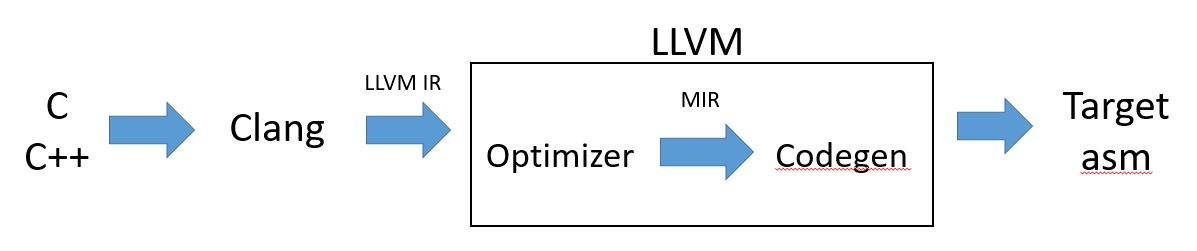
\includegraphics[width=0.9\textwidth]{LLVM.PNG}
  \caption{Упрощённая схема LLVM}
\end{figure}

\subsection{Архитектура ARC}

\indent

Для проверки эффекта, который будут оказывать разрабатываемые трансформации, использовалась целевая архитектура ARC, используемая в emdebbed устройствах. Это специальные процессоры, которые конфигурируются во время синтеза так, чтобы максимально соответствовать назначению. Данная архитектура поддерживается компанией Synopsys\cite{Snps}

В данном проекте использовалась система компиляции MetaWare для архитектуры ARC. Запуск скомпилированных приложений происходил на потактовом симуляторе ARC.

\section{Реализация}

\indent

В ходе работы была реализована трансформация, состоящая из четырёх отдельных фаз, каждая из которых специализируется на одном конкретном виде доступа к данным.

\subsection{Преаллокация}

\indent

% MIPS ISA ref
Инструкция преаллокации, в отличие от инструкции предподкачки, нет так сильно распространена в наборе команд современных процессоров. Например, её реализуют MIPS\cite{MIPS} и ARC, но такой инструкции нет в x86.

\begin{figure}
  \centering
  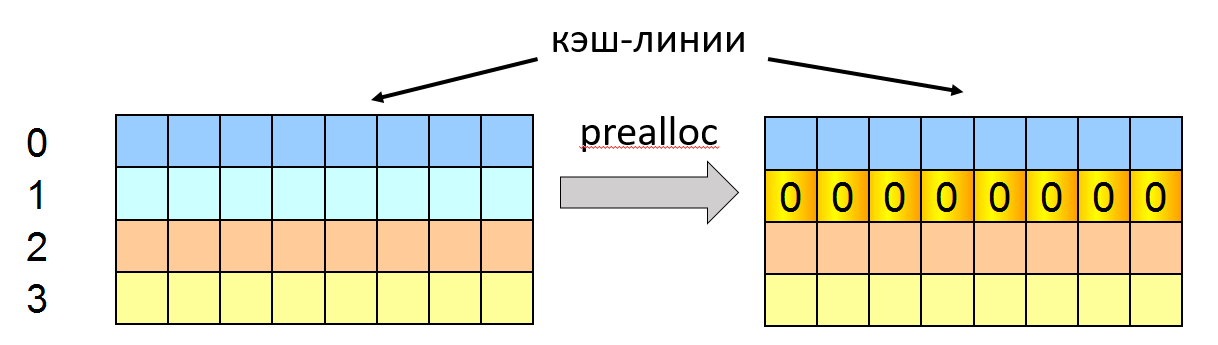
\includegraphics[width=0.9\textwidth]{prealloc.PNG}
  \caption{Схема работы инструкции преаллокации}
\end{figure}


\subsubsection{Архитектурные особенности}

\indent

Перед тем как приступить к обсуждению самого алгоритма, необходимо пояснить, что такое преаллокация. Инструкция преаллокации позволяет выделить целую кэш-линию в ожидании того, что она полностью будет перезаписана. Таким образом снижается нагрузка на пропускную способность памяти, так как происходит всего лишь одно обращение, при котором данные с кэш-линии отправляются в память. Сама кэш-линия после этого просто зануляется. В архитектуре MIPS на линии также выставляются соответствующие флаги. Благодаря такому способу использования кэш-линий нагрузка на память снижается в два раза, по сравнению с обычной предподкачкой данных с использованием специальной инструкции, запрашивающей владение линией.

\subsubsection{Алгоритм}

\indent

Из-за нераспространённости данной инструкции не удалось найти публикаций на тему программной преаллокации кэш-линий. Поэтому алгоритм в этой работе придуман самостоятельно, хотя и не является чем-то сложным. В реализации рассматриваются только самые вложенные циклы.

Основная проблема при вставке преаллокации -- корректность программы. При неострожном использовании инструкции данные в памяти могут занулиться, приведя к неправильному исполнению кода. Поэтому основная часть алгоритма состоит из проверок на корректность применения трансформации.

\lstinputlisting[caption=Алгоритм для преаллокации, style=CStyle]{prealloc.c}

В первую очередь в циклах проверяются все доступы в память. Если присутствует хотя бы одно чтение из памяти -- цикл отбрасывается. У инструкций записи в память сохраняются адреса, для дальнейшего анализа, при этом одновременно сверяется, сколько байт сохраняет инструкция. Если хотя бы одна запись в память имеет другой размер, то анализ цикла прекращается.

После того, как набраны все записи, начинается анализ на полное покрытие кэш-линии. Сначала проверяется, что шаг изменения индуктивной переменной, домноженный на размер записи, равен размеру кэш-линии. Таким образом гарантируется, что на каждой итерации будет использоваться новая кэш-линия. Если это не так, то цикл отбрасывается. Затем проверяется, что все адреса лежат в пределах одной кэш-линии. За этой проверкой следует поиск самого младшего (базового) адреса. Для этого адреса должно выполняться условие, что он выровнен по границе кэш-линии, так как именно его будет использовать инструкция преаллокации. После этого вычисляется, полностью ли инструкции записи в память покрывают кэш-линию. Если да, то в начале цикла вставляется инструкция преаллокации, использующая самый младший адрес.

\subsubsection{Возможности для улучшения}

\indent

Первое, что можно предложить для улучшения фазы, -- это использование дополнительной информации о переменных, например, предположений, заданных программистом. Также возможно добавление директив, сообщающих о том, что в цикле можно безопасно выполнить преаллокацию. Анализ указателей может помочь, если встретятся несколько идентификаторов, которые будут использоваться как адреса для записи в память.

\subsection{Регулярные доступы}

\indent

Следующая подфаза оптимизации обрабатывает обычные регулярные доступы к массивам в тех случаях, когда преаллокация выключена, либо она не сработала. Также на некоторых архитектурах эта оптимизация будет лишней по причине наличия аппаратной поддержки предподкачки данных для регулярных доступов (например, с помощью потокового буфера).

\subsubsection{Существующая фаза}

\indent

В LLVM уже существовала фаза для регулярных доступов. В её функционал входила обработка инструкций чтения из памяти и записи в неё. Псевдокод трансформации приведён в листинге.

\lstinputlisting[caption=Алгоритм для регулярных доступов, style=CStyle]{stride_old.c}

Фаза применяется ко всем самым вложенным циклам в программе. Сначала оценивается количество итераций, на которое будет сдвигаться индекс для предподкачки. После этого анализируется каждая инструкция в цикле.

Всю работу для каждой инструкции можно поделить на три этапа. На первом этапе проверяется, является ли инструкция чтением памяти или записью (в случае записи ещё проверяется опция, контролирующая необходимость предподкачки для таких инструкций) и в случае успеха запоминается её адрес. Во второй части идёт проверка, действительно ли необходимо добавить предподкачку для этого адреса или же ранее уже была добавлена предподкачка для адреса в той же кэш-линии и зависит ли адрес от индуктивной переменной. Если предподкачка не нужна, то фаза переходит к анализу следующей инструкции. На последней стадии уже вставляются сами инструкции предподкачки с вычисленным новым адресом и правильным типом доступа (чтение или запись). Затем исходный адрес добавляется в список обработанных и начинается анализ следующей инструкции.

\subsubsection{Добавленные возможности}

\indent

В рамках данной работы существующая фаза была расширена в двух направлениях.

Во-первых, появилась возможность включать предподкачку для внешних циклов. Данное изменение не потребовало большой модификации кода и не представляет особого интереса, так как не имеет какой-либо алгоритмической части.

Во-вторых, добавилась вставка предподкачки перед циклом для начальных доступов к массивам. Это расширение потребовало небольшой модификации исходной фазы -- запоминаться стали не только сами адреса, но и тип доступа (запись или чтение). Затем с помощью собранной информации вставляются предподкачки перед циклом по следующему алгоритму.

\lstinputlisting[caption=Алгоритм для предподкачки перед циклом, style=CStyle]{stride_new.c}

Сам алгоритм довольно прост. Для каждого адреса вычисляется его начальный адрес (с начальным значением индуктивной переменной) и затем перед входом в цикл вставляется инструкция предподкачки.

\subsubsection{Возможности для улучшения}

\indent

В ходе работы над улучшением фазы были реализованы не все важные дополнения. В качестве дальнейшей работы в этом направлении можно выделить несколько существенных моментов. Во-первых, необходимо добавить дополнительный анализ на применимость оптимизации, например, используя анализ указателей, чтобы не генерировать лишние инструкции. Во-вторых, очень важно использовать профильную информацию, показывающую, какие места требуют оптимизации, а какие нет.

\subsection{Косвенные доступы}

\indent

Третьей частью большой оптимизации стала предподкачка для косвенных доступов. В исследованных компиляторах эта фаза реализована только в Oracle C/C++ Compiler. В LLVM трансформация разрабатывалась с нуля, став самой сложной и объёмной частью из всех четырёх подфаз. Оптимизация рассматривает только самые вложенные циклы.

\subsubsection{Базовый алгоритм}

\indent

За основу взят алгоритм, упоминавшийся в подразделе об исследованиях программных методов предподкачки для косвенных доступов\cite{AinsworthIA}. Однако при реализации алгоритм претерпел изменения и в нём появились новые стадии. Первая добавленная стадия -- поиск индуктивных переменных, вторая -- поиск граничных условий для найденных переменных, следующие две -- те же самые, что и в публикации, а последняя является расширением стадии из алгоритма.

Рассмотрим сначала две оставшиеся теми же самыми фазы. Листинг поиска в глубину приведён далее.

\lstinputlisting[caption=Поиск цепочки загрузок обходом графа потока данных в глубину, style=CStyle]{indirect_stage_2.c}

В качестве входных параметров функции подаются инструкция загрузки, пустая цепочка для дальнейшего заполнения и найденные ранее индуктивные переменные. Исполнение начинается с цикла, сканирующего операнды инструкции. Рассмаривается три случая: если операнд -- индуктивная переменная, то поиск по этому пути заканчивается успешно; если операнд является инвариантом цикла, то поиск по данному пути заканчивается неудачей; в остальных случаях рекурсивно вызывается поиск в глубину. В случае успеха цикл прерывается, инструкция добавляется в цепочку и поиск завершается успешно. В противном случае проверяется следующий операнд. Если по всем путям поиск оказался неуспешным, то цепочка остаётся пустой.

После отработки этой процедуры для инструкции загрузки получается готовая цепочка, начиная от первой операции над индуктивной переменной и заканчивая самим чтением из памяти.

Третья фаза проще. В ней сливаются пересекающиеся цепочки (например, цепочка с одной загрузкой и цепочка с двумя, первая из которых из первой цепочки) и отбрасываются неподходящие цепочки, включающие в себя $\phi$-узлы или вызовы функций, а также если хотя бы одно чтение не доминирует инструкцию, изменяющую индуктивную переменную.

Последняя фаза -- это непосредственно генерация кода. Каждая цепочка проходится столько раз, сколько в ней загрузок. На каждой итерации генерируется код для предподкачки со сдвинутым на определённое число индексом. Когда цикл доходит до самой инструкции загрузки, вместо неё добавляется предподкачка. После этого цикл начинается заново для следующей инструкции загрузки, уже использующую предыдущую, как индекс. При этом сдвинутые индексы для промежуточный чтений из памяти проверяются на правильность сравнением с граничным значением индуктивной переменной. Если индекс больше этого значения, то предподкачка идёт адресу с граничным значением.

\subsubsection{Расширенная версия}

\indent

В этой части будут подробно разобраны дополнительные и модифицированные стадии.

\paragraph{Поиск базовых индуктивных переменных}

Поиск базовых индуктивных переменных необходим для упрощения и ускорения последующего этапа поиска цепочек. Для каждой найденной переменной создаётся специальный дескриптор, включающий в себя саму переменную, инструкцию для её изменения, инструкцию сравнения на выход из цикла и максимальное значение этой переменной. Алгоритм распознавания индуктивных переменных приведён в листинге.

\lstinputlisting[caption=Проверка\, является ли $\phi$-узел индуктивной переменной, style=CStyle]{indirect_stage_1.c}

Вся проверка состоит из достаточно простых шагов. Сначала проверяется количество операндов -- в алгоритме рассматриваются только простые индуктивные переменные и циклы без сложного графа потока управления, поэтому у $\phi$-узла должно быть два операнда -- один приходит извне цикла, второй -- следующее значение этой переменной. Затем проверяется, как получено следующее значение. Во-первых, это должна быть разрешённая операция (одна из простых операций, например, сложение), во-вторых, шаг должен быть инвариантом цикла, в-третьих, оставшимся операндом должна быть исходный $\phi$-узел. Если все условия удовлетворяются, для переменной заводится дескриптор.

После этого ищется условие выхода из цикла для данной индуктивной переменной. Алгоритм на псевдокоде приведён далее.

\lstinputlisting[caption=Поиск условия для выхода из цикла, style=CStyle]{indirect_stage_1_cmp.c}

Сначала проверяется, находится ли следующее значение индуктивной переменной внутри линейного участка с выходом из цикла. Если проверка успешна, то анализируется инструкция перехода в начало цикла. Она должна быть условной и сравнение для неё должно содержать инвариант цикла (граничное значение индуктивной переменной) и следующее значение индуктивной переменной. В случае прохождения всех проверок дескриптор индуктивной переменной обновляется.

Дескриптор индуктивной переменной запоминается, только если обе функции успешно отработали. В противном случае переменная отбрасывается.

\paragraph{Случаи с шагом большим единицы и неизвестным на этапе компиляции шагом}

Улучшение алгоритма в этом случае достигается за счёт изменения схемы, по которой генерируется конечный код. Если шаг не равен единице, то выбор максимального значения затрудняется тем, что нельзя утверждать, что, например, вычитание шага из граничного значения даст правильный индекс (например, проход по всем чётным индексам при границе, равной 999 -- шаг равен двум, максимальное значение -- 998). Поэтому в таком случае необходимо менять способ получения нового индекса.

Для этого вводятся дополнительные индуктивные переменные, изменяющиеся с тем же шагом, что и основная, но имеющие начальное значение, равное сдвигу, который раньше прибавлялся к основной переменной. Также в конце цикла добавляется получение следующих значений дополнительных переменных по аналогии с основной индуктивностью. В таком случае если следующее значение дополнительной переменной превышает границу, то просто берётся старое значение -- увеличения не происходит. Однако данный метод имеет один недостаток -- он повышает давление на регистры.

\paragraph{Вычисление дистанции с учётом сгенерированного кода}

Последним улучшением алгоритма, реализованным в работе, является более точное вычисление дистанции для предподкачки. Формула для получения дистанции выглядит следующим образом:

\begin{displaymath}
  D = \frac{t - i}{t} \times \frac{N}{loop\ size}.
\end{displaymath}

Данная формула отличается от приведённой в публикации тем, что в ней учитывается размер цикла в инструкциях. Сам размер вычисляется уже после того, как трансформация сгенерировала код, чтобы получить наиболее точное значение. После того, как становится известен размер, каждый сгенерированный сдвиг основной индуктивной переменной поправляется с учётом дополнительного кода.

\subsubsection{Возможности для улучшения}

\indent

Дальнейшая работа над этой фазой может включать в себя использование анализа указателей для более точного вычисления применимости оптимизации и учёт профильной информации по промахам в кэш. Также возможно расширение стандартного анализа в LLVM -- скалярной эволюции -- для работы с более сложными инструкциями, такими как загрузки из памяти. Ещё один шаг к улучшению фазы -- учёт давления на регистры. Сейчас в LLVM нет стандартного способа определить этот параметр на этапе машинно-независимых оптимизаций.

\subsection{Рекурсивные структуры данных}

\indent

Последняя часть комплексной оптимизации -- это предподкачка для рекурсивных структур данных. В работе учитывались исследования разных алгоритмов для достижения цели, в результате чего самым подходящим способом оказалась жадная предподкачка. Реализация рассматривает только доступы в самых вложенных циклах.

\subsubsection{Определение рекурсивных структур данных}

\indent

В отличие от алгоритма, приведённого в исследованиях существующих решений, при реализации не учитывались рекурсивные структуры данных с косвенностью. То есть, если в структуре есть указатель на объект того же типа, то она считается рекурсивной. В случае же если указатель является чем-то более сложным, например массивом указателей, или указателем на указатель на какую-то структуру другого типа, то такой тип не рассматривается. Этот подход значительно упрощает анализ, при этом не сильно уменьшая применимость фазы, так как нетривиальные использования указателей для реализации рекурсивных структур данных встречаются реже, чем ссылки в структурах на объекты того же типа.

\subsubsection{Алгоритм}

\indent

Весь алгоритм делится на три стадии.

Первая -- определение адресов для предподкачки. Рассматриваются все загрузки из памяти, в результате которых получается значение того же типа, что и у адреса, используемого этой инструкцией. Таким образом, подтверждается, что идёт обращение к рекурсивной структуре. После этого проверяется, что адрес получается в результате преобразований $\phi$-узла, также имеющего тип указателя на такую структуру. Операндами такого $\phi$-узла являются начальное значение, приходящее снаружи, и указатель на следующий элемент структуры. Если проверка пройдена, то загруженный адрес и $\phi$-узел сохраняются отдельно друг от друга.

Вторая стадия -- это вставка кода для предподкачки в цикле. Для всех сохранённых адресов просто генерируется инструкция предподкачки сразу же после инструкции загрузки адреса из памяти.

Третья стадия -- добавление предподкачки перед циклом для доступа к первому элементу. Для этого из сохранённых $\phi$-узлов выбирается операнд, являющийся начальным значением (инвариант цикла), и для этого адреса перед входом в цикл добавляется предподкачка.

\subsubsection{Возможности для улучшения}

\indent

В качестве улучшений реализованного алгоритма предлагается учитывать профильную информацию для анализа применимости. Вторым изменением можно добавить перестановку инструкций местами, чтобы предподкачка проиходила как можно раньше, а не перед проверкой условия выхода из цикла.

\section{Контроль фаз}

\indent

Разработанная фаза получилась очень большой по своей функциональности. Поэтому для более тонкой настройки каждой отдельной части необходимо организовать интерфейс для пользователя, если он захочет что-нибудь подстроить под себя.

\subsection{Опции}

\indent

Изучение современных компиляторов, проведённое в пределах данной работы, показало, что имеет смысл добавить в компилятор большое количество опций, позволяющих управлять поведением оптимизации.

Весь список новых опций, появившихся после реализации фазы, представлен следующим набором:

\begin{itemize}
\item \texttt{\textbf{-stride-prefetch=\{true|false\}}} -- включение или выключение фазы предподкачки для регулярных доступов;
\item \texttt{\textbf{-cache-line-size=N}} -- задание размера кэш-линии;
\item \texttt{\textbf{-indirect-prefetch=\{true|false\}}} -- включение или выключение фазы предподкачки для косвенных доступов;
\item \texttt{\textbf{-indirect-prefetch-distance=N}} -- задание константы $N$ в формуле для дистанции в косвенных доступах;
\item \texttt{\textbf{-rds-prefetch=\{true|false\}}} -- включение или выключение фазы предподкачки для доступов к рекурсивным структурам данных;
\item \texttt{\textbf{-prefetch-outer-loops=\{true|false\}}} -- включение или выключение предподкачки для регулярных доступов во внешнем цикле;
\item \texttt{\textbf{-use-llvm-prefetch=\{true|false\}}} -- использовать стандартную инструкцию LLVM или специфичные для архитектуры ARC;
\item \texttt{\textbf{-use-all-arc-intrinsic=\{true|false\}}} -- использовать только предподкачку для чтения или ещё и для записи вместе с инструкцией преаллокации.
\end{itemize}

Также одна существующая опция поменяла своё значение:\linebreak
\texttt{\textbf{-loop-prefetch=\{true|false\}}} -- включение или выключение всей фазы;

\subsection{Директивы}

\indent 
Изучение компилятора ICC показало, что удобно давать пользователю возможность управлять фазой на уровне отдельных циклов. Поэтому в компилятор были добавлены директивы на основе уже существующей в LLVM \texttt{\textbf{\#pragma clang loop}}:

\begin{itemize}
\item \texttt{\textbf{\#pragma clang loop prefetch(type)}} -- включение или выключение фазы в определённом цикле;
\item \texttt{\textbf{\#pragma clang loop prefetch(type, var[, var...]}} -- аналогично первой директиве, но с указанием конкретных идентификаторов, которые будут рассматриваться при анализе.
\end{itemize}

Возможные значения для типа директивы следующие:

\begin{itemize}
\item \texttt{\textbf{disable}} -- полное выключение оптимизации;
\item \texttt{\textbf{rds}} -- применение только фазы для рекурсивных структур данных;
\item \texttt{\textbf{array}} -- применение только фазы для регулярных и косвенных доступов;
\item \texttt{\textbf{enable}} -- включение всей оптимизации;
\end{itemize}

\subsection{Аттрибуты}

\indent

Также в качестве дополнительной возможности в компилятор добавлен атрибут для функции:\linebreak
\texttt{\textbf{\_\_attribute\_\_((prefetch(\{enable|disable\})))}} -- включение или выключение оптимизации на уровне отдельной функции.

\section{Тестирование}

Важной частью данной работы стало тестирование и отладка реализованных фаз. Благодаря этому удалось добиться хорошей стабильности оптимизации, а также измерить количество срабатываний на большом наборе тестов.

\subsection{Инфраструктура для тестирования}

Для тестирования использовалось несколько наборов бенчмарков, а также самописные юнит-тесты. Использовались следующие известные бенчмарки.
\begin{itemize}
\item Ливерморские циклы\cite{Liver} -- набор тестов, осуществляющих научные вычисления. Содержит много различных циклов.
\item DSPstone\cite{DSP} -- бенчмарк для встраиваемых систем, состоящих из реализации различных фильтров, преобразования фурье, перемножения матриц.
\item LLVM Nightly Testsuite\cite{LNT} -- большой пакет тестов для проекта LLVM, состоит из разной степени сложности приложений и бенчмарков.
\item Юнит-тесты под архитектуру ARC -- набор тестов, проверяющих применимость трансформаций и их корректность при исполнении.
\item Юнит-тесты для x86 -- тесты на компиляцию и на исполнение на платформе x86.
\end{itemize}

\pagebreak

\subsection{Применимость фаз}

Количество применений фаз измерялось на LLVM Nightly Testuite. Результаты представлены в следующей таблице.

\begin{figure}[h!]
  \centering
  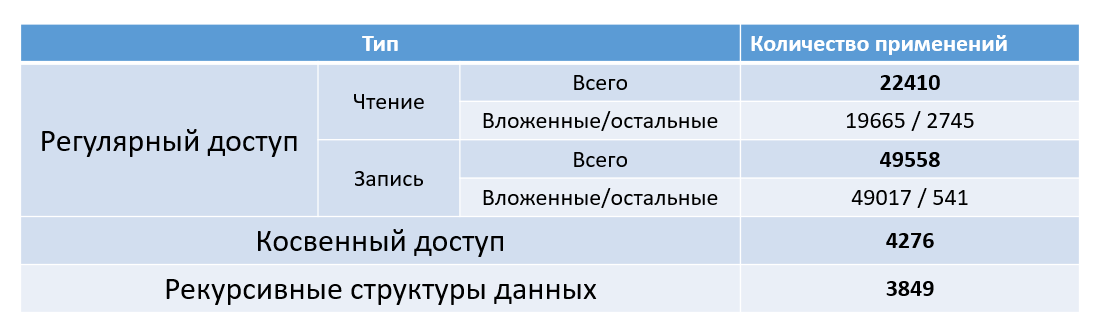
\includegraphics[width=0.9\textwidth]{table_01.PNG}
  \caption{Применимость фаз на LNT}
\end{figure}


\subsection{Покрытие кода}

Покрытие кода измерялось с помощью утилиты gcov на трёх наборах тестов. Результаты представлены в таблице.

\begin{figure}[h!]
  \centering
  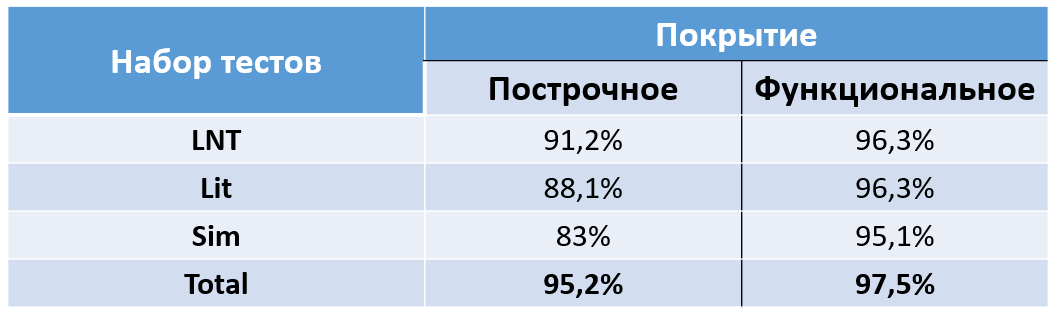
\includegraphics[width=0.9\textwidth]{coverage.PNG}
  \caption{Покрытие разработанных фаз}
\end{figure}


Суммарное покрытие получилось очень хорошим. В таблице видно неполное покрытие по функциям, потому что в коде присутствуют методы, используемые только для отладки.

\newpage

\section{Заключение}

\paragraph{Исследование алгоритмов}

Исследовано 8 различных подходов к ускорению приложений при различных типах доступа. Также проведена классификация шаблонов использования памяти. Результатом этой работы стал выбор алгоритмов для последующей реализации комплексной фазы предподкачки.

\paragraph{Исследование компиляторов}

Исследованы 4 промышленных компилятора, среди которых 2 с открытым исходным кодом и 2 проприетарные с закрытым кодом. В компиляторах GCC, LLVM и ICC не оказалось какой-либо серьёзной поддержки автоматической предподкачки, в то время как в компиляторе от Oracle была реализована предподкачка для косвенных доступов.

\paragraph{Разработка фаз}

Разработана большая оптимизация в компиляторе LLVM, включающая в себя четыре отдельных фазы, каждая из которых отвечает за конкретный вид доступов. Фаза преаллокации обрабатывает записи, позволяя снизить количество запросов к памяти. Три фазы для предподкачки отвечают за ускорение приложений при различных шаблонах использования памяти -- для регулярных и косвенных доступах, а также в случае наличия рекурсивных структур данных.

\paragraph{Добавление опций}

В ходе работы был определён интерфейс для взаимодействия с пользователем посредством опций, директив препроцессора и атрибутов функций. Все добавленные методы контроля над поведением оптимизации задокументированы.

\paragraph{Тестирование фаз}

Все разработанные фазы были хорошо протестированы на нескольких наборах тестов, в том числе больших (LLVM Nightly Testsuite). Фазы отлажены и правильно отрабатывают при различных входных данных.

\newpage
\bibliography{my_biblio}{}
\bibliographystyle{plain}
\end{document}